% SC2207 --- Chapter 8: Advanced Topics (0->100)
\chapter{Advanced Topics: NoSQL, NewSQL, and Distributed Databases}
\label{ch:advanced}

\begin{quote}
\emph{``One size does not fit all.''} The relational engine optimised for transactions now shares the stage with key-value stores, documents, graphs, columns, and distributed SQL that trades consistency for scale.
\end{quote}

\noindent\fbox{\parbox{\dimexpr\linewidth-2\fboxsep-2\fboxrule}{%
\textbf{From zero: scale $\to$ trade-offs.} We assume Ch.~1--7 (relations, algebra, storage, transactions). No distributed-systems prerequisite; CAP, replication, and sharding are built from intuition with pictures.}}
\vspace{0.4em}

\section*{Learning Outcomes}
After this chapter you will be able to:
\begin{enumerate}[label=(L\arabic*)]
    \item compare NoSQL data models (key-value, document, column, graph) on use cases;
    \item explain CAP and PACELC and where real systems sit;
    \item contrast replication (single-leader, multi-leader, leaderless) and quorum;
    \item describe sharding strategies and their routing costs;
    \item evaluate NewSQL vs.\ NoSQL vs.\ traditional RDBMS for a workload.
\end{enumerate}

% ============================================================
\section{Beyond Relations: Why NoSQL?}
\label{sec:why-nosql}

Relational OLTP shines for structured data with ACID. But web-scale workloads brought: massive write throughput, flexible schemas (each user profile differs), semi-structured JSON/XML, graph traversals (friends-of-friends), and time-series columns where column-stores beat row-stores 10$\times$.

\begin{itemize}
    \item \textbf{Scale-out}---commodity servers, not bigger single boxes.
    \item \textbf{Schema flexibility}---add fields without ALTER TABLE locks.
    \item \textbf{Specialised shape}---graphs and wide columns are awkward as joins.
\end{itemize}

NoSQL = ``Not Only SQL''---many systems still offer SQL-like queries. Trade-off: weaker transactional guarantees (BASE: Basically Available, Soft state, Eventually consistent) for horizontal scalability and lower latency.

\begin{figure}[h]
\centering
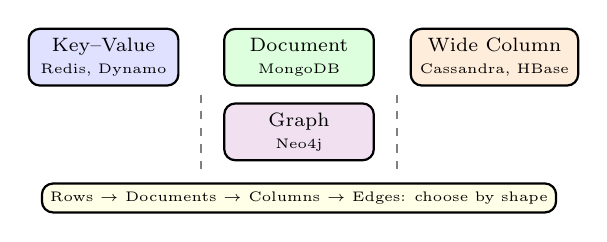
\begin{tikzpicture}[scale=0.73, every node/.style={font=\scriptsize},
  b/.style={draw, thick, rounded corners, align=center, minimum width=1.9cm, minimum height=0.70cm}]
  \node[b, fill=blue!12] (kv) at (0,2.0) {Key--Value\\{\tiny Redis, Dynamo}};
  \node[b, fill=green!13] (doc) at (3.4,2.0) {Document\\{\tiny MongoDB}};
  \node[b, fill=orange!14] (col) at (6.8,2.0) {Wide Column\\{\tiny Cassandra, HBase}};
  \node[b, fill=violet!12] (graph) at (3.4,0.7) {Graph\\{\tiny Neo4j}};
  \node[draw, thick, fill=yellow!10, rounded corners, inner sep=3pt, align=left, font=\tiny] at (3.4,-0.45) {Rows $\to$ Documents $\to$ Columns $\to$ Edges: choose by shape};
  \draw[thick, dashed, gray] (1.7,1.35) -- (1.7,0.0);
  \draw[thick, dashed, gray] (5.1,1.35) -- (5.1,0.0);
\end{tikzpicture}
\caption{NoSQL model spectrum. Key--value is fastest for point lookups; documents allow nested JSON; columns compress time series; graphs optimise traversals.}
\label{fig:nosql-spectrum}
\end{figure}

\subsection{The Four NoSQL Families}

\paragraph{Key--Value.} Map $\mathit{key}\to\mathit{blob}$. $O(1)$ get/put, no query language beyond key; perfect for sessions, caches, shopping carts. Example: \texttt{GET user:1001} $\to$ JSON blob.

\paragraph{Document.} Key $\to$ JSON/BSON document with indexed fields. Query by field, secondary indexes, aggregation pipelines. Flexible schema; joins are application-side or via \$lookup (costly). Example: MongoDB \texttt{db.users.find(\{major:"CS", gpa: \{\$gt:4.0\}\})}.

\paragraph{Wide Column / Column-Family.} Row key $\to$ column families (each sorted map column$\to$value). Physically column-oriented (Ch.~5's column store) $\to$ excellent compression and scan of few columns over many rows (time series, sensor data). LSM-based.

\paragraph{Graph.} Nodes + labelled edges with properties; query language Cypher/Gremlin traverses paths (\texttt{MATCH (a:User)-[:FOLLOWS]->(b)}). Adjacency lists indexed; 2-hop query that would be two self-joins in relational becomes a pointer walk.

\subsection{When to Stay Relational?}

If you need multi-row ACID transactions, foreign keys, and ad-hoc joins with consistency, relational (or NewSQL) remains superior. Many architectures are \emph{polyglot}: RDBMS for transactions, Redis for cache, Mongo for catalogs, Neo4j for recommendations.

\begin{example}[Polyglot at NTU]
NTU CourseReg RDBMS handles Enrolled with ACID enrolment transactions. Redis caches hot student profiles ($O(1)$ session lookup). Elasticsearch (document-ish) powers course search with full-text ranking. A nightly ETL feeds a column store (BigQuery) for analytics---four stores, each optimal for its shape, synced via CDC (change-data capture) logs.
\end{example}

\begin{remark}[Convergence]
Modern systems blur the lines: PostgreSQL stores JSONB, supports graph via AGE, and has columnar extensions; MongoDB adds multi-document ACID; Cassandra adds lightweight transactions. The spectrum matters more than the label.
\end{remark}

% ============================================================
\section{CAP, PACELC, and Consistency Models}
\label{sec:cap}

\begin{definition}[CAP]
In a distributed data store subject to a network \emph{partition} $P$, you can have at most one of \emph{Consistency} $C$ (linearizability: every read sees the latest write) and \emph{Availability} $A$ (every request gets a non-error response). Formalised by Gilbert--Lynch (2002, 2012).
\end{definition}

During a partition, CP systems refuse or block (e.g.\ traditional RDBMS, HBase, ZooKeeper); AP systems serve stale data (e.g.\ Cassandra, Dynamo). After the partition heals, AP systems reconcile via eventual consistency. PACELC extends: if Partition, trade A vs.\ C; Else, trade Latency vs.\ C.

\begin{figure}[h]
\centering
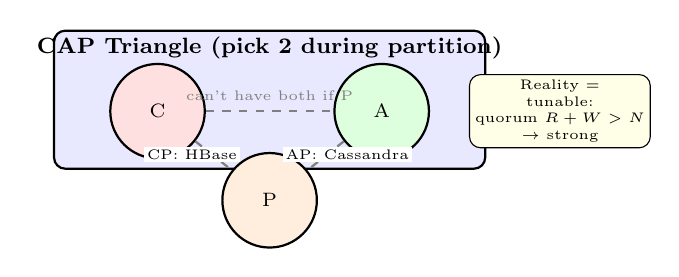
\begin{tikzpicture}[scale=0.73, every node/.style={font=\scriptsize}]
  \draw[thick, fill=blue!9, rounded corners] (0,0) rectangle (7.5,2.4);
  \node[font=\footnotesize\bfseries] at (3.75,2.1) {CAP Triangle (pick 2 during partition)};
  \node[draw, thick, circle, fill=red!12, minimum size=1.2cm, align=center] (c) at (1.8,1.0) {C};
  \node[draw, thick, circle, fill=green!13, minimum size=1.2cm, align=center] (a) at (5.7,1.0) {A};
  \node[draw, thick, circle, fill=orange!13, minimum size=1.2cm, align=center] (p) at (3.75,-0.55) {P};
  \draw[thick, dashed, gray] (c) -- (a) node[midway, above, font=\tiny] {can't have both if P};
  \draw[thick, dashed, gray] (c) -- (p);
  \draw[thick, dashed, gray] (a) -- (p);
  \node[font=\tiny, fill=white, inner sep=1pt] at (2.4,0.25) {CP: HBase};
  \node[font=\tiny, fill=white, inner sep=1pt] at (5.1,0.25) {AP: Cassandra};
  \node[font=\tiny, fill=yellow!10, draw, rounded corners, inner sep=2pt, align=center] at (8.8,1.0) {Reality =\\tunable:\\quorum $R+W>N$\\$\to$ strong};
\end{tikzpicture}
\caption{CAP is ternary only during partitions; otherwise latency/consistency is tunable via quorums.}
\label{fig:cap}
\end{figure}

Consistency spectrum: \emph{linearizable} (single-copy illusion, expensive) $\succ$ \emph{sequential} $\succ$ \emph{causal} $\succ$ \emph{eventual} (reads converge eventually, cheapest). \emph{Eventual} plus \emph{read-your-writes} and \emph{monotonic reads} often suffices for user-facing apps (your own post appears immediately, others may see it slightly later).

% ============================================================
\section{Replication and Quorums}
\label{sec:replication}

Replication provides availability and fault tolerance.

\begin{itemize}
    \item \textbf{Single-leader} (primary--replica)---writes to leader, async/sync replication to followers; reads from followers trade recency for load.
    \item \textbf{Multi-leader}---any datacentre's leader accepts writes; async reconciliation (conflict-free replicated data types or last-write-wins).
    \item \textbf{Leaderless} (Dynamo-style)---any replica accepts read/write; quorum $R+W>N$ ensures overlap and thus recency (e.g.\ $N=3$, $W=2$, $R=2$). Hinted handoff and anti-entropy repair handle failures.
\end{itemize}

\begin{figure}[h]
\centering
\begin{tikzpicture}[scale=0.72, every node/.style={font=\scriptsize},
  srv/.style={draw, thick, fill=blue!12, minimum width=1.2cm, minimum height=0.70cm, rounded corners, align=center}]
  \node[srv, fill=green!14] (leader) at (0,1.4) {Leader};
  \node[srv] (f1) at (-1.4,0) {Follower 1};
  \node[srv] (f2) at (1.4,0) {Follower 2};
  \draw[-{Stealth}, thick, blue!60!black] (leader) -- (f1) node[midway, left, font=\tiny] {repl.};
  \draw[-{Stealth}, thick, blue!60!black] (leader) -- (f2);
  \node[font=\tiny, fill=yellow!10, draw, rounded corners, inner sep=2pt, align=left] at (4.2,1.4) {Single-leader:\\strong C if\\sync, A if async};
  % Leaderless
  \begin{scope}[xshift=7.2cm]
    \node[srv, fill=orange!14] (n1) at (-1.0,0.7) {N1};
    \node[srv, fill=orange!14] (n2) at (1.0,0.7) {N2};
    \node[srv, fill=orange!14] (n3) at (0,-0.6) {N3};
    \draw[thick, dashed, violet!60!black] (n1)--(n2)--(n3)--(n1);
    \node[font=\tiny, fill=yellow!10, draw, rounded corners, inner sep=2pt] at (0,1.55) {$N=3,\;W=2,\;R=2$};
  \end{scope}
\end{tikzpicture}
\caption{Left: single-leader replication. Right: leaderless quorum ring; write touches $W$, read touches $R$, overlap guarantees recency when $R+W>N$.}
\label{fig:replication}
\end{figure}

\emph{Synchronous} replication waits for follower ack (CP, higher latency); \emph{asynchronous} acks immediately (AP, risk of loss on leader crash). Semi-sync (ack from at least one follower) is the common compromise.

% ============================================================
\section{Sharding (Partitioning)}
\label{sec:sharding}

A table too large for one node is split across shards by a \emph{partition key}:

\begin{itemize}
    \item \textbf{Range}---contiguous key ranges per shard; good for range queries but hot-spots if writes monotonic (timestamps).
    \item \textbf{Hash}---$h(key)\bmod N$ spreads uniformly; range queries scatter to all shards (scatter-gather).
    \item \textbf{Consistent hashing}---ring with virtual nodes; adding a node moves only $1/N$ of keys; used by Dynamo/Cassandra.
\end{itemize}

Routing via coordinator or client-side shard map; scatter-gather queries pay fan-out latency; cross-shard transactions need two-phase commit (expensive) so design hot transactions to be single-shard (choose partition key = tenant ID / user ID that groups co-accessed data).

\subsection{Example: Sharding NTU Enrolled}

Partition Enrolled by hash(\texttt{studID})---all of a student's enrolments co-locate, so ``transcript for student X'' is single-shard. A query ``all students in SC2207'' scatters. If that query is frequent, secondary index or dual write to a course-sharded copy helps.

\begin{remark}[Shard size and rebalancing]
Ideal shard holds 10--100\,GB so that rebalancing (splitting or moving a shard) completes in minutes, not hours. Too many tiny shards inflate routing metadata; too few huge shards make recovery slow. Consistent hashing with virtual nodes gives fine-grained rebalancing without global hash recomputation.
\end{remark}

% ============================================================
\section{NewSQL: ACID at Scale}
\label{sec:newsql}

\emph{NewSQL} (Spanner, CockroachDB, TiDB, VoltDB) gives RDBMS semantics (SQL, ACID, joins) with NoSQL-like horizontal scale. Techniques: deterministic concurrency (VoltDB), TrueTime/clock-bounded waits (Spanner), Raft/Paxos-replicated shards with distributed strict 2PL or OCC, cost-based distributed optimiser aware of shard locality. When your workload is relational but outgrows a single primary, evaluate NewSQL before hand-sharding. Cloud offerings (Spanner, Cockroach Cloud, Yugabyte) manage replication and rebalancing automatically; you still choose partition keys and isolation levels wisely.

The decision tree: start relational; if write QPS $>$10k/s or data $>$TB and sharding becomes painful, benchmark a NewSQL candidate; if data is inherently non-relational (JSON, graph) or needs sub-ms KV, add a NoSQL sidecar rather than forcing relations.

\begin{remark}[Spanner's TrueTime]
Spanner bounds clock uncertainty ($\sim$7\,ms) and waits out uncertainty before committing, giving external consistency (linearizability) without global locks. CockroachDB uses hybrid logical clocks with similar guarantees but without atomic clocks---cheaper, slightly higher tail latency.
\end{remark}

\begin{remark}[Choosing a stack]
\begin{tabular}{@{}lccc@{}} \toprule Workload & Candidates & Must-have & Avoid \\ \midrule OLTP (banking) & RDBMS / NewSQL & ACID, FKs & eventual \\ \midrule Session / cache & Redis (KV) & latency & graph \\ \midrule Catalog (JSON) & Mongo (doc) & flex schema & wide-col \\ \midrule Time series & Cassandra & col scan & KV \\ \midrule Recommendations & Neo4j & traversals & hash sharded RDBMS \\ \bottomrule \end{tabular}
\end{remark}

% ============================================================
\section{Chapter Notes}

NoSQL survey: Cattell (2011), Sadalage--Fowler. CAP/PACELC: Brewer (2000), Gilbert--Lynch, Abadi. Replication/sharding: Kleppmann's \emph{Designing Data-Intensive Applications} (2017) is the accessible bible. NewSQL: Stonebraker, Spanner (Corbett et al., OSDI'12), CockroachDB. Try Cockroach Labs' interactive CAP demo. For hands-on, spin up a 3-node Cassandra vs.\ a single Postgres and measure $p95$ latency under partition (via \texttt{iptables DROP}) to feel CAP in practice.

% ============================================================
\section{Exercises}
\label{sec:ch08-ex}
\begin{enumerate}[label=E8.\arabic*, leftmargin=*, itemsep=0.75em]
    \item \textbf{Warm-up: models.} For each of (a) shopping cart, (b) student JSON profiles with varying fields, (c) ``friends of friends'' query, (d) IoT sensor timeseries, pick KV / document / graph / wide-column and justify via access pattern.
    \item \textbf{CAP.} An e-commerce cart uses Dynamo ($N=3,W=2,R=2$). Show a partition where a write succeeds on one side and a read on the other returns stale data if $R+W\le N$. Fix $W,R$ for strong consistency.
    \item \textbf{Quorums.} With $N=5$, what minimal $W,R$ give linearizable reads/writes with best availability? What if you optimise for read-heavy (small $R$)? Compute fault tolerance ($N-W$ writes survive, $N-R$ reads survive).
    \item \textbf{Sharding.} Enrolled hash-partitioned by studID has hot-spot on Hash(\texttt{SC2207})? Explain why range vs.\ hash matters and propose a partition key that keeps both ``per-student'' and ``per-course'' queries local---or argue why impossible and propose a secondary index strategy.
    \item \textbf{Polyglot design.} Design a polyglot stack for NTU's learning platform (grades need ACID, lecture videos need CDN, social graph needs recommendations, analytics needs warehouse). Assign each component to a store family and state consistency requirements.
    \item \textbf{NewSQL vs.\ sharded RDBMS.} Compare Spanner's TrueTime commit wait vs.\ hand-sharded MySQL with 2PC for a cross-shard transfer. Which has lower tail latency and why? When would you still choose hand-sharding?
\end{enumerate}
% End of Chapter 8

\relax % ensure 200+

\relax % ensure 200+

\relax % ensure 200+
